\section{Các bài kiểm tra khác}

\subsection{IQ Test}
Chỉ số thông minh IQ là từ viết tắt của từ *Intelligence Quotient*, thường được xem là có liên quan mật thiết tới thành công của một người trong cuộc sống, trong công việc và trong vấn đề học tập. 

Căn cứ vào rất nhiều nghiên cứu, những người có chỉ số IQ cao được xem là những người có khả năng thực hành, xử lý và phân tích chuỗi thông tin ở mức độ chuyên sâu hơn và tốc độ nhanh hơn so với những người có chỉ số IQ thấp hơn. 

Công cụ đo IQ là những bài kiểm tra trắc nghiệm, hiện là phương pháp phổ biến nhất được nhiều tổ chức trên thế giới sử dụng. Dựa vào kết quả bài kiểm tra, chỉ số IQ của mỗi cá nhân sẽ được phân loại như sau:
\begin{itemize}
    \item Chỉ số IQ dưới 85: thuộc loại thấp (khoảng 16\% dân số).
    \item Chỉ số IQ từ 85-115: thuộc loại bình thường (chiếm khoảng 68\% dân số).
    \item Chỉ số IQ từ 115-130: thuộc loại thông minh (chiếm khoảng 14\% dân số).
    \item Chỉ số IQ từ 130-145: thuộc loại rất thông minh (chiếm khoảng 2\% dân số).
    \item Chỉ số IQ trên 145: thuộc loại thiên tài hoặc cận thiên tài (chiếm khoảng 0.1\% dân số).
\end{itemize}

Bài kiểm tra IQ trong hệ thống bao gồm các câu hỏi logic, toán học, và hình học. Dưới đây là danh sách các câu hỏi trong bài kiểm tra:

\begin{multicols}{2}
\noindent
\textbf{Câu 1:} Trước nửa đêm là bao nhiêu phút nếu trước đó 32 phút thời gian này gấp 3 lần số phút sau 22 giờ? \\
A. 18 \\
B. 22 \\
C. 24 \\
D. 20 \\

\textbf{Câu 2:} Cho dãy số: 2 8 18 32 50 ? Số nào có thể thay vào chỗ có dấu hỏi chấm? \\
A. 60 \\
B. 70 \\
C. 64 \\
D. 72 \\

\textbf{Câu 3:} Trong một gia đình có sáu thành viên A, B, C, D, E và F. A và B là một cặp vợ chồng, A là thành viên nam. D là con trai duy nhất của C. C là anh trai của A. E là em gái của D. B là con dâu của F. F có chồng đã chết. Có bao nhiêu thành viên nam trong gia đình? \\
A. 2 \\
B. 4 \\
C. 3 \\
D. 5 \\

\textbf{Câu 4:} Ký tự tiếp theo trong dãy sau đây là ký tự nào: A…C…F…J…O…? \\
A. S \\
B. T \\
C. U \\
D. V \\

\textbf{Câu 5:} Mối quan hệ giữa cháu gái với cháu trai thì tương tự như anh em trai với: \\
A. Cha mẹ \\
B. Chị em gái \\
C. Anh em họ \\
D. Chị em họ \\

\textbf{Câu 6:} Simon thuê một chiếc xe hơi đi từ thành phố lên núi cách đó 100 km để trượt tuyết. Giữa đường, cô đón người bạn Nina, và tiếp tục đi 50 km còn lại với cô này. Lúc về, Simon dừng lại nhà Nina để cho cô xuống, và Simon về nhà một mình. Simon phải trả 50 USD thuê xe và 10 USD tiền xăng. Nếu tính sòng phẳng ra, thì Nina phải trả bao nhiêu tiền? \\
A. 15 \\
B. 20 \\
C. 25 \\
D. 30 \\

\textbf{Câu 7:} Số tiếp theo trong dãy số sau đây là số nào: 144 121 ...100 81 64? \\
A. 45 \\
B. 49 \\
C. 53 \\
D. 57 \\

\textbf{Câu 8:} Nếu từ WOLF tương ứng với số 8526, thì từ FLOW tương ứng với số nào sau đây? \\
A. 2856 \\
B. 6258 \\
C. 5862 \\
D. 6852 \\

\textbf{Câu 9:} Hương ra khỏi nhà với 90.000 đồng trong túi. Cô chi tiêu hết 1/3 số tiền ở siêu thị và tiếp tục chi 1/3 số tiền còn lại ở nhà thuốc. Nếu Hương không chi thêm khoản nào khác thì khi về nhà trong túi cô còn bao nhiêu tiền? \\
A. 30.000 \\
B. 40.000 \\
C. 33.000 \\
D. 50.000 \\

\textbf{Câu 10:} Trong một buổi cắm trại gồm 100 học sinh, nhà trường chuẩn bị trang phục cho học sinh gồm 40 áo màu trắng, 60 áo màu xanh và 70 quần màu trắng, 30 quần màu xanh. Nhà trường sẽ phát áo và quần ngẫu nhiên cho các học sinh. Như vậy sẽ có: \\
A. Ít nhất 20 học sinh mặc cả áo lẫn quần màu trắng. \\
B. Ít nhất 20 học sinh mặc cả áo lẫn quần màu xanh. \\
C. Ít nhất 10 học sinh mặc cả áo lẫn quần màu trắng. \\
D. Ít nhất 10 học sinh mặc cả áo lẫn quần màu xanh. \\

\textbf{Câu 11:} Một cầu thủ sút bóng vào cầu môn hai lần độc lập nhau. Biết rằng xác suất sút trúng vào cầu môn của cầu thủ đó là 0,7. Xác suất sao cho cầu thủ đó sút một lần trượt và một lần trúng cầu môn là: \\
A. 1 \\
B. 0,7 \\
C. 0,42 \\
D. 0,21 \\

\textbf{Câu 12:} Biết rằng 1/2 của số tiền trong một quỹ tín thác được đầu tư vào cổ phiếu, 1/4 được đầu tư vào trái phiếu và 1/5 được đầu tư vào các quỹ tương hỗ, còn lại 10.000\$ đầu tư vào công trái chính phủ. Hỏi tổng số tiền của quỹ tín thác là bao nhiêu? \\
A. 100.000\$ \\
B. 150.000\$ \\
C. 200.000\$ \\
D. 250.000\$ \\

\textbf{Câu 13:} Cho mệnh đề sai: "Nếu là bạn của Tuấn thì biết bơi". Hỏi trong các mệnh đề dưới đây, mệnh đề nào đúng? \\
A. Nếu không biết bơi thì là bạn của Tuấn. \\
B. Nếu không biết bơi thì không là bạn của Tuấn. \\
C. Nếu không là bạn của Tuấn thì biết bơi. \\
D. Nếu biết bơi thì là không là bạn của Tuấn. \\

\textbf{Câu 14:} An cao hơn Tuấn, Bình không cao bằng An, Đức thấp hơn Tuấn. Hỏi phát biểu nào sau đây là đúng nhất? \\
A. Tuấn cao hơn Bình. \\
B. Bình cao hơn Tuấn. \\
C. Đức cao hơn An. \\
D. Chưa đủ cơ sở để kết luận Tuấn hay Bình cao hơn. \\

\textbf{Câu 15:} Tìm số tiếp theo của dãy sau: 5 25 29 85 89? \\
A. 135 \\
B. 145 \\
C. 120 \\
D. 133 \\

\textbf{Câu 16:} Nhà Thanh có ao bèo 1.000m\textsuperscript{2}, ngày hôm sau số lượng bèo sẽ nở gấp đôi ngày hôm trước, đến ngày thứ 18 thì bèo đã nở được nửa ao. Vậy đến ngày thứ bao nhiêu thì bèo sẽ nở đầy ao? \\
A. Ngày thứ 19 \\
B. Ngày thứ 20 \\
C. Ngày thứ 21 \\
D. Ngày thứ 22 \\

\textbf{Câu 17:} Số tiếp theo của dãy số 1, 1, 2, 3, 5? \\
A. 6 \\
B. 7 \\
C. 8 \\
D. 9 \\

\textbf{Câu 18:} FBG\_, GBF\_, HBI\_, IBH\_ \_\_\_\_ Điền vào chỗ trống? \\
A. HBL \\
B. HBK \\
C. JBK \\
D. JBI \\

\textbf{Câu 19:} Số tiếp theo của chuỗi số 0, 1, 2, 4, 6, 9, 12, 16, ? \\
A. 18 \\
B. 20 \\
C. 22 \\
D. 24 \\

\textbf{Câu 20:} Số nào khác tính chất với những số còn lại 9678 4572 5261 5133 3527 6895 7768? \\
A. 9678 \\
B. 4572 \\
C. 3527 \\
D. 7768 \\

\end{multicols}


\subsection{EQ Test}
EQ (Emotional Quotient) hay còn gọi là trí tuệ cảm xúc, đo lường khả năng nhận biết, quản lý và điều chỉnh cảm xúc cá nhân cũng như tương tác với cảm xúc của người khác. Những người có EQ cao thường giữ được sự bình tĩnh trong các tình huống áp lực, biết cách xây dựng các mối quan hệ tốt đẹp và đưa ra quyết định đúng đắn.

Trong bài kiểm tra EQ của hệ thống, điểm số sẽ được phân chia như sau:
\begin{itemize}
    \item \textbf{Dưới 85}: Thuộc nhóm người có EQ thấp, khả năng sáng tạo và quản lý cảm xúc bị hạn chế.
    \item \textbf{Từ 85 đến 115}: Đây là mức phổ biến nhất, phản ánh khả năng cảm xúc ở mức trung bình.
    \item \textbf{Từ 116 đến 131}: Thuộc nhóm người có EQ cao, dễ dàng kiểm soát cảm xúc và sáng tạo.
    \item \textbf{Trên 131}: Là nhóm rất ít người đạt được, thể hiện khả năng cảm xúc đặc biệt vượt trội.
\end{itemize}
Bài kiểm tra EQ sử dụng các tình huống thực tế để đánh giá khả năng ứng phó, sáng tạo và xử lý cảm xúc của người dùng.


Bộ câu hỏi của bài test như sau:

\begin{multicols}{2}
\noindent
\textbf{Câu 1:} Khi đang ngồi trên máy bay, đột nhiên máy bay rung động rất mạnh và lắc lư qua trái phải. Lúc đó, bạn sẽ làm gì? \\
A. Tiếp tục xem điện thoại, không quan tâm. \\
B. Quan sát tình hình thay đổi, cẩn thận lắng nghe thông báo từ tiếp viên. \\
C. Cả A và B đều đúng. \\
D. Tôi không biết, tôi không quan tâm. \\

\textbf{Câu 2:} Có một đứa trẻ trong nhóm 4 đứa mà bạn đang trông nom khóc vì không ai chơi cùng. Bạn sẽ làm gì lúc này? \\
A. Không quan tâm. \\
B. Trò chuyện, tìm cách giúp đứa trẻ. \\
C. Nhắc nhở bé nín khóc. \\
D. Cho bé đồ chơi. \\

\textbf{Câu 3:} Bạn là sinh viên và muốn đạt điểm cao ở môn học A, nhưng kết quả bài thi giữa kỳ môn đó chỉ ở mức trung bình. Bạn sẽ làm gì? \\
A. Lập kế hoạch học tập và quyết tâm thực hiện. \\
B. Sau này sẽ học tập chăm chỉ hơn. \\
C. Khích lệ bản thân: môn này không tốt thì tập trung vào môn học khác. \\
D. Thuyết phục giảng viên cho điểm cao hơn. \\

\textbf{Câu 4:} Bạn là nhân viên bán bảo hiểm và đang tìm kiếm khách hàng mới. Cả 15 người bạn trao đổi đều không có thái độ rõ ràng hoặc không muốn hợp tác. Lúc đó, bạn sẽ làm gì? \\
A. Nghĩ chuyện này chỉ xảy ra hôm nay, hy vọng ngày mai sẽ may mắn hơn. \\
B. Xem xét lại mình có phù hợp với công việc không. \\
C. Cố gắng hơn ở buổi gặp sau, duy trì thái độ làm việc siêng năng. \\
D. Bỏ qua 15 người này và tìm khách hàng khác. \\

\textbf{Câu 5:} Bạn là giám đốc và đưa ra quy định không được phân biệt chủng tộc trong công ty. Một hôm, bạn vô tình nghe thấy có người pha trò về vấn đề này. Bạn sẽ giải quyết như thế nào? \\
A. Mặc kệ, đó chỉ là trò đùa. \\
B. Gọi người đó vào phòng và mắng anh ta. \\
C. Ngay lập tức nói với anh ta rằng công ty không chấp nhận những trò đùa như vậy. \\
D. Khuyên người đó tham gia khóa học chống phân biệt chủng tộc. \\

\textbf{Câu 6:} Bạn thân bạn đang lái xe thì đột nhiên bị xe của người khác tông vào, khiến anh ấy rất tức giận. Bạn sẽ làm gì để anh ấy bình tĩnh trở lại? \\
A. Khuyên ngăn anh ấy bỏ qua. Không ai bị thương, không có vấn đề gì lớn. \\
B. Chuyển sự chú ý bằng một bài hát anh ấy thích. \\
C. Cùng anh ấy đổ lỗi cho người lái xe kia, thể hiện rằng bạn đứng về phía anh ấy. \\
D. Kể với anh ấy trải nghiệm tương tự của bạn. Lúc đó bạn cũng rất tức giận, nhưng sau đó bạn thấy tài xế bị tai nạn và được đưa đi cấp cứu. \\

\textbf{Câu 7:} Bạn và chồng/vợ mâu thuẫn dẫn đến cãi nhau gay gắt. Trong lúc nóng nảy, cả hai đã xô xát với nhau, dù hai bạn thực sự không muốn. Lúc đó, bạn sẽ làm gì? \\
A. Im lặng 20 phút sau đó tiếp tục tranh luận. \\
B. Ngừng tranh cãi, im lặng mặc cho dù đối phương nói gì. \\
C. Xin lỗi đối phương và yêu cầu anh ấy/cô ấy xin lỗi. \\
D. Dừng lại sắp xếp suy nghĩ, sau đó trình bày quan điểm của bạn. \\

\textbf{Câu 8:} Bạn là trưởng bộ phận và muốn đề xuất biện pháp để giải quyết các vấn đề trong công việc. Vậy bạn sẽ làm gì trước tiên? \\
A. Sắp xếp lịch họp mỗi ngày để tối đa hóa thời gian thảo luận với mọi người. \\
B. Cho mọi người thời gian để tìm hiểu nhau. \\
C. Yêu cầu từng người chia sẻ cách giải quyết vấn đề. \\
D. Khuyến khích mọi người chia sẻ nhiều ý tưởng sáng tạo. \\

\textbf{Câu 9:} Con trai 3 tuổi của bạn rất nhút nhát. Bé sợ người lạ và sợ đến những nơi xa lạ. Bạn sẽ làm gì? \\
A. Chấp nhận tính nhút nhát của trẻ, xem xét cách để bé tránh được những nơi cảm thấy không được thoải mái. \\
B. Đưa con đến gặp chuyên gia tâm lý. \\
C. Cố tình đưa con đi gặp nhiều người, đến những nơi xa lạ để con vượt qua nỗi sợ. \\
D. Lên kế hoạch cho con học cách đối phó với người lạ theo mức độ tăng dần. \\

\textbf{Câu 10:} Bạn muốn bắt đầu học lại loại nhạc cụ đã từng học khi còn nhỏ. Bạn sẽ làm gì để tận dụng tối đa thời gian? \\
A. Luyện tập đều đặn mỗi ngày. \\
B. Lựa chọn bản nhạc có thể cải thiện khả năng của bạn để luyện tập. \\
C. Chỉ tập nếu có hứng thú. \\
D. Chọn bản nhạc khó hơn so với khả năng nhưng nếu bạn luyện tập nhiều thì vẫn chơi được. \\
\end{multicols}

\subsection{Trắc nghiệm 3 thiên hướng học tập}

Trắc nghiệm 3 thiên hướng học tập VAK là một bài tập trắc nghiệm nhằm xác định thiên hướng học tập của người dùng. Mô hình VAK cho rằng mỗi cá nhân có một cách học tập lý tưởng và đạt được các hiệu quả học tập khác nhau. Khái niệm VAK lần đầu tiên được phát triển bởi các nhà tâm lý học và các chuyên gia giảng dạy trẻ em, bao gồm Fernald, Keller, Orton, Gillingham, Stillman và Montessori từ những năm 1920.

Mô hình phong cách học tập VAK thông qua bài trắc nghiệm gồm 20 câu hỏi, giúp đánh giá phong cách học tập ưa thích của người dùng, từ đó xác định tỷ lệ giữa ba thiên hướng học tập cơ bản: trực quan, thính giác và xúc giác. Kết quả trắc nghiệm sẽ phản ánh tỷ lệ phần trăm của từng thiên hướng, từ đó người dùng có thể biết được thiên hướng học tập ưu tiên của mình.

Dựa trên kết quả trắc nghiệm, VAK tiếp tục thiết kế phương pháp học tập và các loại trải nghiệm phù hợp cho từng cá nhân, giúp tối ưu hóa quá trình học tập và phát triển cá nhân.

Đặc Điểm Của Các Thiên Hướng Học Tập Chính:
\begin{itemize}
    \item \textbf{Visual - Trực Quan:} Liên quan đến việc sử dụng những thứ đã nhìn thấy hoặc quan sát được, bao gồm hình ảnh, sơ đồ, minh họa, màn hình, tài liệu phát tay, phim,... Thiên hướng học tập này phù hợp với những người học tốt thông qua việc quan sát và có khả năng xử lý thông tin tốt thông qua việc đọc biểu đồ và dựa trên hình ảnh minh họa để hiểu rõ các khái niệm bài học.
    \item \textbf{Auditory - Thính Giác:} Liên quan đến việc tiếp nhận thông tin qua âm thanh: từ những gì được nói, từ bản thân hoặc người khác, âm thanh và tiếng ồn. Những người có thiên hướng thính giác học tốt thông qua việc lắng nghe, chẳng hạn như trong các bài giảng trên lớp hoặc các hướng dẫn bằng lời.
    \item \textbf{Kinesthetic - Xúc Giác:} Liên quan đến trải nghiệm thể chất bao gồm: chạm, cảm nhận, cầm nắm và thực hành. Những người học theo thiên hướng xúc giác thường học tốt thông qua các hoạt động thực hành, làm dự án, tham gia các bài tập nhóm, hoặc trải nghiệm thực tế, và đặc biệt họ áp dụng kiến thức qua các thí nghiệm hoặc tự tay thực nghiệm để rút ra kiến thức.
\end{itemize}

\begin{multicols}{2}
\noindent
\textbf{Câu 1:} Bạn muốn đọc loại sách nào để giải trí? \\
A. Một cuốn sách có nhiều hình ảnh. \\
B. Một cuốn sách có rất nhiều từ trong đó. \\
C. Một cuốn sách có trò chơi tìm kiếm từ hoặc ô chữ. \\

\textbf{Câu 2:} Khi bạn không chắc chắn về cách đánh vần một từ, bạn có xu hướng làm gì nhất? \\
A. Viết ra để xem có đúng không. \\
B. Đánh vần lớn tiếng để xem nghe có đúng không. \\
C. Dò theo từng chữ cái trên không (đánh vần bằng tay). \\

\textbf{Câu 3:} Bạn đang mua quần áo và đứng chờ thanh toán. Bạn có xu hướng làm gì trong khi chờ đợi? \\
A. Nhìn quanh các bộ quần áo khác trên giá. \\
B. Nói chuyện với người đứng cạnh bạn trong hàng. \\
C. Cử động tay chân hoặc di chuyển qua lại. \\

\textbf{Câu 4:} Khi bạn thấy từ 'mèo', điều đầu tiên bạn làm là gì? \\
A. Hình dung một con mèo trong tâm trí bạn. \\
B. Tự nói từ 'mèo' với chính mình. \\
C. Nghĩ về việc ở cùng một con mèo (vuốt ve hoặc nghe tiếng mèo kêu). \\

\textbf{Câu 5:} Cách tốt nhất để bạn ôn tập cho một bài kiểm tra là gì? \\
A. Đọc sách hoặc ghi chú của bạn và xem lại các biểu đồ hoặc hình ảnh. \\
B. Nhờ ai đó hỏi bạn các câu hỏi mà bạn có thể trả lời thành tiếng. \\
C. Tạo thẻ ghi nhớ mà bạn có thể ôn lại. \\

\textbf{Câu 6:} Cách tốt nhất để bạn học cách sử dụng một thứ gì đó (như máy tính hoặc trò chơi điện tử) là gì? \\
A. Nhờ ai đó chỉ cho bạn. \\
B. Đọc hoặc nghe ai đó giải thích. \\
C. Tự mình tìm cách làm. \\

\textbf{Câu 7:} Nếu bạn tham dự một buổi khiêu vũ ở trường, bạn sẽ nhớ điều gì nhất vào ngày hôm sau? \\
A. Khuôn mặt của những người đã có mặt. \\
B. Bản nhạc đã được chơi. \\
C. Những điệu nhảy bạn đã thực hiện và thức ăn bạn đã ăn. \\

\textbf{Câu 8:} Bạn thấy điều gì làm bạn mất tập trung nhất khi bạn đang cố gắng học? \\
A. Mọi người đi ngang qua bạn. \\
B. Tiếng ồn lớn. \\
C. Ghế ngồi không thoải mái. \\

\textbf{Câu 9:} Khi bạn tức giận, bạn có xu hướng làm gì nhất? \\
A. Thể hiện khuôn mặt 'tức giận' của bạn. \\
B. La hét. \\
C. Đập cửa. \\

\textbf{Câu 10:} Khi bạn vui vẻ, bạn có xu hướng làm gì nhất? \\
A. Cười toe toét. \\
B. Nói không ngừng. \\
C. Hành động rất phấn khích. \\
\textbf{Câu 11:} Khi đến một nơi mới, bạn sẽ tìm đường như thế nào? \\
A. Tìm bản đồ hoặc sơ đồ chỉ ra mọi thứ. \\
B. Hỏi ai đó chỉ đường. \\
C. Cứ bắt đầu đi loanh quanh cho đến khi tìm thấy thứ bạn cần. \\

\textbf{Câu 12:} Trong ba lớp học sau, bạn yêu thích lớp nào nhất? \\
A. Lớp học nghệ thuật. \\
B. Lớp học âm nhạc. \\
C. Lớp thể dục. \\

\textbf{Câu 13:} Khi bạn nghe một bài hát trên radio, bạn có xu hướng làm gì nhất? \\
A. Hình dung video đi kèm với bài hát. \\
B. Hát hoặc ngân nga theo nhạc. \\
C. Bắt đầu nhảy và gõ nhịp chân. \\

\textbf{Câu 14:} Điều gì làm bạn mất tập trung nhất khi đang trong lớp học? \\
A. Ánh sáng quá sáng hoặc quá tối. \\
B. Tiếng ồn từ hành lang hoặc bên ngoài tòa nhà (như giao thông hoặc ai đó đang cắt cỏ). \\
C. Nhiệt độ quá nóng hoặc quá lạnh. \\

\textbf{Câu 15:} Bạn thích làm gì để thư giãn? \\
A. Đọc sách. \\
B. Nghe nhạc. \\
C. Tập thể dục (đi bộ, chạy, chơi thể thao, v.v.). \\

\textbf{Câu 16:} Cách tốt nhất để bạn nhớ số điện thoại của một người bạn là gì? \\
A. Hình dung các số trên điện thoại như khi bạn quay số. \\
B. Nói to nhiều lần. \\
C. Viết ra hoặc lưu vào danh bạ điện thoại. \\

\textbf{Câu 17:} Nếu bạn thắng một trò chơi, bạn sẽ chọn phần thưởng nào trong ba phần thưởng sau? \\
A. Một tấm poster treo tường. \\
B. Thẻ quà tặng dịch vụ nghe nhạc trực tuyến. \\
C. Một trò chơi nào đó (hoặc một quả bóng đá, bóng rổ, v.v.). \\

\textbf{Câu 18:} Bạn thích đi đâu với nhóm bạn của mình hơn? \\
A. Xem phim. \\
B. Buổi hòa nhạc. \\
C. Công viên giải trí. \\

\textbf{Câu 19:} Bạn có xu hướng nhớ điều gì nhất về những người mới gặp? \\
A. Khuôn mặt của họ nhưng không nhớ tên. \\
B. Tên của họ nhưng không nhớ khuôn mặt. \\
C. Những gì bạn đã nói chuyện với họ. \\

\textbf{Câu 20:} Khi bạn chỉ đường cho ai đó đến nhà mình, bạn có xu hướng nói gì nhất? \\
A. Mô tả các tòa nhà và địa danh họ sẽ đi qua. \\
B. Tên của các con đường hoặc đường phố họ sẽ đi qua. \\
C. 'Đi theo tôi - sẽ dễ hơn nếu tôi chỉ cho bạn cách đến đó.\\
\end{multicols}


\subsection{Trắc nghiệm Não Trái - Não Phải}

Trắc nghiệm "Não Trái - Não Phải" là một công cụ nghiên cứu nhằm khám phá sự phân bổ và hoạt động của hai bán cầu não, từ đó hiểu rõ hơn về xu hướng tư duy và cách thức xử lý thông tin của mỗi cá nhân. Dựa trên lý thuyết về sự khác biệt giữa bán cầu não trái và não phải, bài trắc nghiệm này cung cấp một cái nhìn sâu sắc về các đặc điểm nhận thức, tư duy và cách con người tương tác với môi trường xung quanh.

\begin{itemize}
  \item \textbf{Não Trái:} Bán cầu não trái chủ yếu liên quan đến các chức năng tư duy logic, phân tích, tổ chức, và xử lý thông tin theo trình tự. Người thuận não trái thường giỏi trong việc sử dụng ngôn ngữ, làm việc khoa học, tính toán, ghi nhớ, và có khả năng nhận thức thời gian tốt. Những cá nhân này có xu hướng kỷ luật, thích lên kế hoạch và xử lý công việc theo cách có tổ chức.
  
  \item \textbf{Não Phải:} Bán cầu não phải chịu trách nhiệm cho khả năng sáng tạo, trí tưởng tượng và cảm xúc. Người thuận não phải thường có năng khiếu trong các lĩnh vực nghệ thuật, trực giác mạnh mẽ và khả năng thích ứng với những tình huống không xác định. Những cá nhân này thường cảm nhận và phản ứng với thế giới qua cảm xúc và trực giác, thích hợp với các công việc sáng tạo như nghệ sĩ, nhà văn, hay nhà thiết kế.
\end{itemize}

Thông qua bài trắc nghiệm đơn giản này, bạn sẽ biết được tuổi não trái và não phải, đâu là thế mạnh nên phát huy của bản thân.
\begin{itemize}
  \item \textbf{Người thuận não trái:} Đây là những người có lượng neuron thần kinh được phân bổ ở bán cầu não trái nhiều hơn so với bán cầu não phải. Họ có khả năng tư duy logic, phân tích chi tiết, và khả năng tổ chức, phân loại thông tin tốt. Những người này thường có tính kỷ luật cao và thường xuyên xử lý thông tin theo cách tuần tự và có cấu trúc.
  
  \item \textbf{Người thuận cả hai bán cầu não:} Những người này có sự kết hợp giữa lý trí và logic của bán cầu não trái, đồng thời sở hữu trực giác và khả năng sáng tạo của bán cầu não phải. Họ có thể giải quyết vấn đề từ cả hai góc độ, sử dụng khả năng phân tích cũng như sáng tạo trong công việc và cuộc sống.
  
  \item \textbf{Người thuận não phải:} Đây là những người có số lượng neuron thần kinh nhiều hơn ở bán cầu não phải. Những người này thường được miêu tả là giàu cảm xúc, có trực giác sắc bén và óc sáng tạo cao. Họ thường có xu hướng làm việc trong các lĩnh vực nghệ thuật, sáng tạo hoặc những công việc đòi hỏi khả năng tư duy tự do. Các cá nhân này thường có khả năng cảm nhận sâu sắc và nhận diện được các tín hiệu không lời, như việc nhận diện sự giả dối hay những hành động không trung thực.
\end{itemize}

Bộ câu hỏi của bài test như sau:
\begin{multicols}{2}
\noindent
\textbf{Câu 1:} Chọn mô tả đúng nhất với bản thân: \\
A. Ở nhà, phòng của tôi có ngăn kéo và tủ được tổ chức gọn gàng. Tôi cũng cố gắng sắp xếp những thứ khác quanh nhà. \\
B. Ở nhà, tôi thích phong cách sống tự nhiên, thoải mái. Tôi dọn dẹp khi thấy cần thiết và khi có thời gian. \\

\textbf{Câu 2:} Chọn mô tả đúng nhất với bản thân: \\
A. Bàn làm việc của tôi thường sạch sẽ và mọi thứ đều ở đúng chỗ. \\
B. Tôi để dự án của mình trên bàn để có thể làm việc khi có ý tưởng. \\

\textbf{Câu 3:} Tôi thích: \\
A. Sử dụng phương pháp đã được kiểm chứng và đáng tin cậy. \\
B. Tạo ra những phương pháp mới. \\

\textbf{Câu 4:} Chọn mô tả đúng nhất với bản thân: \\
A. Tôi làm theo hướng dẫn một cách cẩn thận khi xây dựng mô hình, làm đồ thủ công, v.v. \\
B. Tôi thích xây dựng mô hình theo cách của mình, tạo ra sản phẩm riêng. \\

\textbf{Câu 5:} Chọn mô tả đúng nhất với bản thân: \\
A. Tôi hoàn thành một dự án tại một thời điểm. \\
B. Tôi thích bắt đầu nhiều dự án khác nhau, nhưng không thích hoàn thành chúng. \\

\textbf{Câu 6:} Khi tôi được yêu cầu viết một báo cáo về một chủ đề, tôi sẽ: \\
A. Nghiên cứu thông tin, sau đó lập dàn bài và tổ chức bài viết của mình. \\
B. Làm việc theo cảm hứng của riêng mình. \\

\textbf{Câu 7:} Khi tôi phải thực hiện một dự án trong lớp, tôi sẽ: \\
A. sử dụng dự án minh họa trong sách hoặc mô phỏng dự án của một học sinh từng nhận được điểm A+ từ giáo viên của tôi. \\
B. thích thử thách, và như một "nhà khoa học điên", tôi tạo ra một dự án độc đáo. \\

\textbf{Câu 8:} Khi tôi phụ trách một công việc lớn với nhiều người làm việc, tôi thường: \\
A. Tổ chức, giao trách nhiệm cho mọi người, lập danh sách và đảm bảo mọi người hoàn thành phần việc đúng thời hạn. \\
B. Làm việc theo tốc độ của riêng mình, để người khác làm việc theo cách họ muốn. Tôi muốn giải quyết các nhu cầu/vấn đề khi chúng phát sinh. \\

\textbf{Câu 9:} Bạn thích hoạt động nào nhất? \\
A. Lập kế hoạch chi tiết cho một chuyến đi/dự án. \\
B. Tạo ra một hình thức nghệ thuật độc đáo. \\

\textbf{Câu 10:} Tôi rất ghét khi người khác: \\
A. Không quyết đoán về các hoạt động khi tôi ở cùng họ. \\
B. Lên kế hoạch chi tiết từng bước cho các hoạt động khi tôi ở cùng họ. \\

\textbf{Câu 11:} Nếu bạn có thể chọn một bài tập làm văn để thực hiện, bạn sẽ chọn: \\
A. Mô tả các hành tinh trong hệ mặt trời. \\
B. Viết một câu chuyện về một con kiến cứu thế giới. \\

\textbf{Câu 12:} Bạn bè của bạn có khả năng sẽ bầu chọn bạn là: \\
A. Người có khả năng phát minh ra cỗ máy thời gian. \\
B. Người có khả năng bị lạc đường nhất. \\

\textbf{Câu 13:} Buổi sáng bạn mặc đồ dựa theo: \\
A. Bộ trang phục bạn đã lên kế hoạch. \\
B. Bộ nào có mùi ổn là được. \\

\textbf{Câu 14:} Nếu bạn có hai dự án bài tập về nhà cùng lúc, bạn sẽ tiếp tục bằng cách: \\
A. Hoàn thành một cái rồi chuyển sang cái tiếp theo. \\
B. Làm một chút cho một cái đến khi chán, rồi chuyển sang cái kia. \\

\textbf{Câu 15:} Trong một vở kịch, bạn muốn: \\
A. Làm đạo diễn. \\
B. Làm diễn viên chính. \\

\textbf{Câu 16:} Bạn vừa trúng thưởng một kỳ nghỉ miễn phí một tuần đến bãi biển! Bạn sẽ: \\
A. Dành chút thời gian lên kế hoạch cho chuyến đi. \\
B. Đi ngay bây giờ! \\

\textbf{Câu 17:} Ai đó vừa nói với bạn rằng bạn có khả năng ngoại cảm. Bạn nghĩ: \\
A. Điều đó thật vô lý. \\
B. Tôi nghĩ có thể mình thật sự có. \\

\textbf{Câu 18:} Trong một bài kiểm tra trắc nghiệm, bạn thường: \\
A. Xem xét các lựa chọn và nhìn ra câu trả lời đúng rõ ràng. \\
B. Suy nghĩ quá nhiều và bị rối. \\

\textbf{Câu 19:} Nếu bạn xem một bộ phim buồn trong lớp, bạn sẽ: \\
A. Kiềm chế cảm xúc. \\
B. Khóc một chút. \\

\textbf{Câu 20:} Khi bạn ăn kẹo M\&M, bạn bị thu hút bởi việc? \\
A. Phân loại theo màu và ăn theo thứ tự. \\
B. Lén ăn trong lớp khi bạn cảm thấy chán. \\

\end{multicols}

\subsection{Trắc nghiệm 5 yếu tố tính cách (Big Five Personality)}

Trắc nghiệm Big Five Personality (hay còn gọi là trắc nghiệm 5 yếu tố tính cách) là một phương pháp được sử dụng rộng rãi trong tâm lý học để đo lường 5 đặc điểm tính cách chủ yếu của một cá nhân. Những đặc điểm này bao gồm:

\begin{itemize}
    \item \textbf{Extraversion (E)}: Đo lường mức độ xã hội, năng động và thích tìm kiếm những trải nghiệm mới mẻ. Người có điểm cao thường thích giao tiếp và tham gia vào các hoạt động xã hội.
    \item \textbf{Agreeableness (A)}: Đo lường mức độ dễ chịu, thân thiện và quan tâm đến người khác. Người có điểm cao dễ đồng cảm và hợp tác với người khác.
    \item \textbf{Conscientiousness (C)}: Đo lường mức độ có tổ chức, chăm chỉ và đáng tin cậy. Người có điểm cao thường rất cẩn thận và thích hoàn thành công việc đúng hạn.
    \item \textbf{Neuroticism (N)}: Đo lường mức độ cảm xúc, dễ bị căng thẳng và dễ thay đổi tâm trạng. Người có điểm cao thường xuyên cảm thấy lo âu hoặc lo lắng.
    \item \textbf{Openness to Experience (O)}: Đo lường mức độ sáng tạo, trí tò mò và sự cởi mở đối với những ý tưởng mới. Người có điểm cao thường thích khám phá và tìm hiểu những điều mới mẻ.
\end{itemize}

Trắc nghiệm năm yếu tố tính cách được thiết kế để giúp bạn hiểu rõ hơn về những đặc điểm tính cách của mình và cách chúng ảnh hưởng đến hành vi, mối quan hệ và cách bạn tương tác với thế giới xung quanh. Sau khi hoàn thành bài kiểm tra, bạn sẽ nhận được điểm số cho từng yếu tố và đánh giá mức độ của các đặc điểm tính cách này.

Căn cứ vào điểm số của người dùng trong từng yếu tố sẽ cho ra kết quả với các mức độ sau:
\begin{itemize}
    \item \textbf{Điểm cao trong Extraversion (E)}: Bạn là người năng động, thích giao tiếp và tham gia vào các hoạt động xã hội.
    \item \textbf{Điểm cao trong Agreeableness (A)}: Bạn là người hòa đồng, dễ gần và quan tâm đến cảm xúc của người khác.
    \item \textbf{Điểm cao trong Conscientiousness (C)}: Bạn là người có tổ chức, chú trọng chi tiết và luôn hoàn thành nhiệm vụ đúng thời gian.
    \item \textbf{Điểm cao trong Neuroticism (N)}: Bạn có thể dễ bị căng thẳng hoặc lo âu, nhưng điều này cũng có thể là động lực để bạn cải thiện bản thân.
    \item \textbf{Điểm cao trong Openness to Experience (O)}: Bạn có trí tò mò, sáng tạo và luôn tìm kiếm sự mới mẻ trong cuộc sống.
\end{itemize}

Bài kiểm tra yêu cầu người dùng đánh giá mức độ từ "Hoàn toàn không đồng ý" đến "Hoàn toàn đồng ý" cho những câu hỏi đánh giá về tính cách của người dùng

\begin{multicols}{2}
\noindent
\textbf{Câu 1:} Tôi là tâm điểm của bữa tiệc. \\
A. Hoàn toàn không đồng ý \\
B. Không đồng ý \\
C. Trung lập \\
D. Đồng ý \\
E. Hoàn toàn đồng ý \\

\textbf{Câu 2:} Tôi ít quan tâm đến người khác. \\
A. Hoàn toàn không đồng ý \\
B. Không đồng ý \\
C. Trung lập \\
D. Đồng ý \\
E. Hoàn toàn đồng ý \\

\textbf{Câu 3:} Tôi luôn chuẩn bị sẵn sàng. \\
A. Hoàn toàn không đồng ý \\
B. Không đồng ý \\
C. Trung lập \\
D. Đồng ý \\
E. Hoàn toàn đồng ý \\

\textbf{Câu 4:} Tôi dễ bị căng thẳng. \\
A. Hoàn toàn không đồng ý \\
B. Không đồng ý \\
C. Trung lập \\
D. Đồng ý \\
E. Hoàn toàn đồng ý \\

\textbf{Câu 5:} Tôi có vốn từ vựng phong phú. \\
A. Hoàn toàn không đồng ý \\
B. Không đồng ý \\
C. Trung lập \\
D. Đồng ý \\
E. Hoàn toàn đồng ý \\

\textbf{Câu 6:} Tôi không nói nhiều. \\
A. Hoàn toàn không đồng ý \\
B. Không đồng ý \\
C. Trung lập \\
D. Đồng ý \\
E. Hoàn toàn đồng ý \\

\textbf{Câu 7:} Tôi quan tâm đến mọi người. \\
A. Hoàn toàn không đồng ý \\
B. Không đồng ý \\
C. Trung lập \\
D. Đồng ý \\
E. Hoàn toàn đồng ý \\

\textbf{Câu 8:} Tôi hay để đồ đạc lung tung. \\
A. Hoàn toàn không đồng ý \\
B. Không đồng ý \\
C. Trung lập \\
D. Đồng ý \\
E. Hoàn toàn đồng ý \\

\textbf{Câu 9:} Tôi thường thư giãn, thoải mái. \\
A. Hoàn toàn không đồng ý \\
B. Không đồng ý \\
C. Trung lập \\
D. Đồng ý \\
E. Hoàn toàn đồng ý \\

\textbf{Câu 10:} Tôi khó hiểu các ý tưởng trừu tượng. \\
A. Hoàn toàn không đồng ý \\
B. Không đồng ý \\
C. Trung lập \\
D. Đồng ý \\
E. Hoàn toàn đồng ý \\

\textbf{Câu 11:} Tôi cảm thấy thoải mái khi ở xung quanh mọi người. \\
A. Hoàn toàn không đồng ý \\
B. Không đồng ý \\
C. Trung lập \\
D. Đồng ý \\
E. Hoàn toàn đồng ý \\

\textbf{Câu 12:} Tôi thường xúc phạm người khác. \\
A. Hoàn toàn không đồng ý \\
B. Không đồng ý \\
C. Trung lập \\
D. Đồng ý \\
E. Hoàn toàn đồng ý \\

\textbf{Câu 13:} Tôi chú ý đến các chi tiết. \\
A. Hoàn toàn không đồng ý \\
B. Không đồng ý \\
C. Trung lập \\
D. Đồng ý \\
E. Hoàn toàn đồng ý \\

\textbf{Câu 14:} Tôi lo lắng về mọi thứ. \\
A. Hoàn toàn không đồng ý \\
B. Không đồng ý \\
C. Trung lập \\
D. Đồng ý \\
E. Hoàn toàn đồng ý \\

\textbf{Câu 15:} Tôi có trí tưởng tượng sống động. \\
A. Hoàn toàn không đồng ý \\
B. Không đồng ý \\
C. Trung lập \\
D. Đồng ý \\
E. Hoàn toàn đồng ý \\

\textbf{Câu 16:} Tôi giữ mình ở phía sau. \\
A. Hoàn toàn không đồng ý \\
B. Không đồng ý \\
C. Trung lập \\
D. Đồng ý \\
E. Hoàn toàn đồng ý \\

\textbf{Câu 17:} Tôi thông cảm với cảm xúc của người khác. \\
A. Hoàn toàn không đồng ý \\
B. Không đồng ý \\
C. Trung lập \\
D. Đồng ý \\
E. Hoàn toàn đồng ý \\

\textbf{Câu 18:} Tôi làm lộn xộn mọi thứ. \\
A. Hoàn toàn không đồng ý \\
B. Không đồng ý \\
C. Trung lập \\
D. Đồng ý \\
E. Hoàn toàn đồng ý \\

\textbf{Câu 19:} Tôi hiếm khi cảm thấy buồn. \\
A. Hoàn toàn không đồng ý \\
B. Không đồng ý \\
C. Trung lập \\
D. Đồng ý \\
E. Hoàn toàn đồng ý \\

\textbf{Câu 20:} Tôi không quan tâm đến các ý tưởng trừu tượng. \\
A. Hoàn toàn không đồng ý \\
B. Không đồng ý \\
C. Trung lập \\
D. Đồng ý \\
E. Hoàn toàn đồng ý \\

\textbf{Câu 21:} Tôi bắt đầu các cuộc trò chuyện. \\
A. Hoàn toàn không đồng ý \\
B. Không đồng ý \\
C. Trung lập \\
D. Đồng ý \\
E. Hoàn toàn đồng ý \\

\textbf{Câu 22:} Tôi không quan tâm đến vấn đề của người khác. \\
A. Hoàn toàn không đồng ý \\
B. Không đồng ý \\
C. Trung lập \\
D. Đồng ý \\
E. Hoàn toàn đồng ý \\

\textbf{Câu 23:} Tôi hoàn thành công việc ngay lập tức. \\
A. Hoàn toàn không đồng ý \\
B. Không đồng ý \\
C. Trung lập \\
D. Đồng ý \\
E. Hoàn toàn đồng ý \\

\textbf{Câu 24:} Tôi dễ bị làm phiền. \\
A. Hoàn toàn không đồng ý \\
B. Không đồng ý \\
C. Trung lập \\
D. Đồng ý \\
E. Hoàn toàn đồng ý \\

\textbf{Câu 25:} Tôi có những ý tưởng tuyệt vời. \\
A. Hoàn toàn không đồng ý \\
B. Không đồng ý \\
C. Trung lập \\
D. Đồng ý \\
E. Hoàn toàn đồng ý \\

\textbf{Câu 26:} Tôi ít nói. \\
A. Hoàn toàn không đồng ý \\
B. Không đồng ý \\
C. Trung lập \\
D. Đồng ý \\
E. Hoàn toàn đồng ý \\

\textbf{Câu 27:} Tôi có ít điều để nói. \\
A. Hoàn toàn không đồng ý \\
B. Không đồng ý \\
C. Trung lập \\
D. Đồng ý \\
E. Hoàn toàn đồng ý \\

\textbf{Câu 28:} Tôi có một trái tim mềm mại. \\
A. Hoàn toàn không đồng ý \\
B. Không đồng ý \\
C. Trung lập \\
D. Đồng ý \\
E. Hoàn toàn đồng ý \\

\textbf{Câu 29:} Tôi dễ bị lo âu. \\
A. Hoàn toàn không đồng ý \\
B. Không đồng ý \\
C. Trung lập \\
D. Đồng ý \\
E. Hoàn toàn đồng ý \\

\textbf{Câu 30:} Tôi thường quên để đồ vật ở đúng chỗ. \\
A. Hoàn toàn không đồng ý \\
B. Không đồng ý \\
C. Trung lập \\
D. Đồng ý \\
E. Hoàn toàn đồng ý \\

\textbf{Câu 31:} Tôi nói chuyện với nhiều người khác nhau tại các bữa tiệc. \\
A. Hoàn toàn không đồng ý \\
B. Không đồng ý \\
C. Trung lập \\
D. Đồng ý \\
E. Hoàn toàn đồng ý \\

\textbf{Câu 32:} Tôi không thực sự quan tâm đến người khác. \\
A. Hoàn toàn không đồng ý \\
B. Không đồng ý \\
C. Trung lập \\
D. Đồng ý \\
E. Hoàn toàn đồng ý \\

\textbf{Câu 33:} Tôi thích sự ngăn nắp. \\
A. Hoàn toàn không đồng ý \\
B. Không đồng ý \\
C. Trung lập \\
D. Đồng ý \\
E. Hoàn toàn đồng ý \\

\textbf{Câu 34:} Tôi thay đổi tâm trạng rất nhanh. \\
A. Hoàn toàn không đồng ý \\
B. Không đồng ý \\
C. Trung lập \\
D. Đồng ý \\
E. Hoàn toàn đồng ý \\

\textbf{Câu 35:} Tôi nhanh chóng hiểu mọi thứ. \\
A. Hoàn toàn không đồng ý \\
B. Không đồng ý \\
C. Trung lập \\
D. Đồng ý \\
E. Hoàn toàn đồng ý \\

\textbf{Câu 36:} Tôi không thích thu hút sự chú ý đến mình. \\
A. Hoàn toàn không đồng ý \\
B. Không đồng ý \\
C. Trung lập \\
D. Đồng ý \\
E. Hoàn toàn đồng ý \\

\textbf{Câu 37:} Tôi dành thời gian cho người khác. \\
A. Hoàn toàn không đồng ý \\
B. Không đồng ý \\
C. Trung lập \\
D. Đồng ý \\
E. Hoàn toàn đồng ý \\

\textbf{Câu 38:} Tôi né tránh trách nhiệm. \\
A. Hoàn toàn không đồng ý \\
B. Không đồng ý \\
C. Trung lập \\
D. Đồng ý \\
E. Hoàn toàn đồng ý \\

\textbf{Câu 39:} Tôi hay bị kích động. \\
A. Hoàn toàn không đồng ý \\
B. Không đồng ý \\
C. Trung lập \\
D. Đồng ý \\
E. Hoàn toàn đồng ý \\

\textbf{Câu 40:} Tôi sử dụng các từ ngữ phức tạp. \\
A. Hoàn toàn không đồng ý \\
B. Không đồng ý \\
C. Trung lập \\
D. Đồng ý \\
E. Hoàn toàn đồng ý \\

\textbf{Câu 41:} Tôi không ngại trở thành trung tâm của sự chú ý. \\
A. Hoàn toàn không đồng ý \\
B. Không đồng ý \\
C. Trung lập \\
D. Đồng ý \\
E. Hoàn toàn đồng ý \\

\textbf{Câu 42:} Tôi cảm nhận được cảm xúc của người khác. \\
A. Hoàn toàn không đồng ý \\
B. Không đồng ý \\
C. Trung lập \\
D. Đồng ý \\
E. Hoàn toàn đồng ý \\

\textbf{Câu 43:} Tôi tuân theo một thời gian biểu. \\
A. Hoàn toàn không đồng ý \\
B. Không đồng ý \\
C. Trung lập \\
D. Đồng ý \\
E. Hoàn toàn đồng ý \\

\textbf{Câu 44:} Tôi dễ dàng bị kích động. \\
A. Hoàn toàn không đồng ý \\
B. Không đồng ý \\
C. Trung lập \\
D. Đồng ý \\
E. Hoàn toàn đồng ý \\

\textbf{Câu 45:} Tôi dành thời gian để suy ngẫm về mọi thứ. \\
A. Hoàn toàn không đồng ý \\
B. Không đồng ý \\
C. Trung lập \\
D. Đồng ý \\
E. Hoàn toàn đồng ý \\

\textbf{Câu 46:} Tôi im lặng khi ở cạnh người lạ. \\
A. Hoàn toàn không đồng ý \\
B. Không đồng ý \\
C. Trung lập \\
D. Đồng ý \\
E. Hoàn toàn đồng ý \\

\textbf{Câu 47:} Tôi làm cho người khác cảm thấy thoải mái. \\
A. Hoàn toàn không đồng ý \\
B. Không đồng ý \\
C. Trung lập \\
D. Đồng ý \\
E. Hoàn toàn đồng ý \\

\textbf{Câu 48:} Tôi làm việc rất cẩn thận và chính xác. \\
A. Hoàn toàn không đồng ý \\
B. Không đồng ý \\
C. Trung lập \\
D. Đồng ý \\
E. Hoàn toàn đồng ý \\

\textbf{Câu 49:} Tôi thường cảm thấy buồn. \\
A. Hoàn toàn không đồng ý \\
B. Không đồng ý \\
C. Trung lập \\
D. Đồng ý \\
E. Hoàn toàn đồng ý \\

\textbf{Câu 50:} Tôi có nhiều ý tưởng. \\
A. Hoàn toàn không đồng ý \\
B. Không đồng ý \\
C. Trung lập \\
D. Đồng ý \\
E. Hoàn toàn đồng ý \\
\end{multicols}

\subsection{Trắc nghiệm phong cách làm việc}

Bài kiểm tra Phong Cách Làm Việc giúp người dùng nhận biết phong cách làm việc chủ đạo của bản thân, cách tiếp cận công việc và tương tác với đồng nghiệp. Qua đó, người dùng sẽ hiểu rõ hơn về điểm mạnh của bản thân và cách tối ưu hóa hiệu quả làm việc trong môi trường công sở.

Bài kiểm tra này phân chia phong cách làm việc thành bốn nhóm chính, mỗi nhóm đại diện cho một kiểu cách làm việc khác nhau, bao gồm:

\begin{itemize}
    \item \textbf{Người Thúc Đẩy:} Sáng tạo, nhiệt tình và thích khám phá những ý tưởng mới. Những người thuộc nhóm này làm việc hiệu quả nhất trong môi trường linh hoạt, sáng tạo và sẵn sàng chấp nhận rủi ro. Họ thường đóng vai trò tiên phong trong các dự án và sáng kiến mới.
    \item \textbf{Người Hỗ Trợ:} Hợp tác, trung thành và nhạy cảm. Người thuộc nhóm này coi trọng cảm xúc và tạo sự hòa hợp trong công việc. Họ luôn sẵn sàng giúp đỡ đồng nghiệp và thường là những người xây dựng mối quan hệ gắn bó trong nhóm.
    \item \textbf{Người Phân Tích:} Logic, tổ chức và kỷ luật. Những người thuộc nhóm này làm việc hiệu quả theo quy trình, yêu thích sự rõ ràng và chi tiết. Họ thích phân tích sâu và đưa ra quyết định dựa trên dữ liệu cụ thể và chính xác.
    \item \textbf{Người Kiểm Soát:} Quyết đoán, tự tin và định hướng kết quả. Những người thuộc nhóm này thích đảm nhận trách nhiệm và có khả năng tập trung vào mục tiêu cụ thể. Họ chủ động trong việc đưa ra quyết định và đạt được các mục tiêu đã đề ra.
\end{itemize}

Việc hoàn thành bài kiểm tra này sẽ giúp người dùng:

\begin{itemize}
    \item Nhận diện phong cách làm việc cá nhân của mình.
    \item Phát huy điểm mạnh và điều chỉnh phương pháp làm việc để đạt hiệu quả cao hơn.
    \item Tạo sự hòa hợp với các phong cách làm việc khác trong môi trường nhóm, từ đó tối ưu hóa hiệu quả công việc chung.
\end{itemize}

Người dùng sẽ lần lượt chọn các ô mô tả tính cách giống với bản thân mình. Bộ câu hỏi của bài kiểm tra có cấu trúc như dưới đây

\begin{figure}[H]
    \centering
    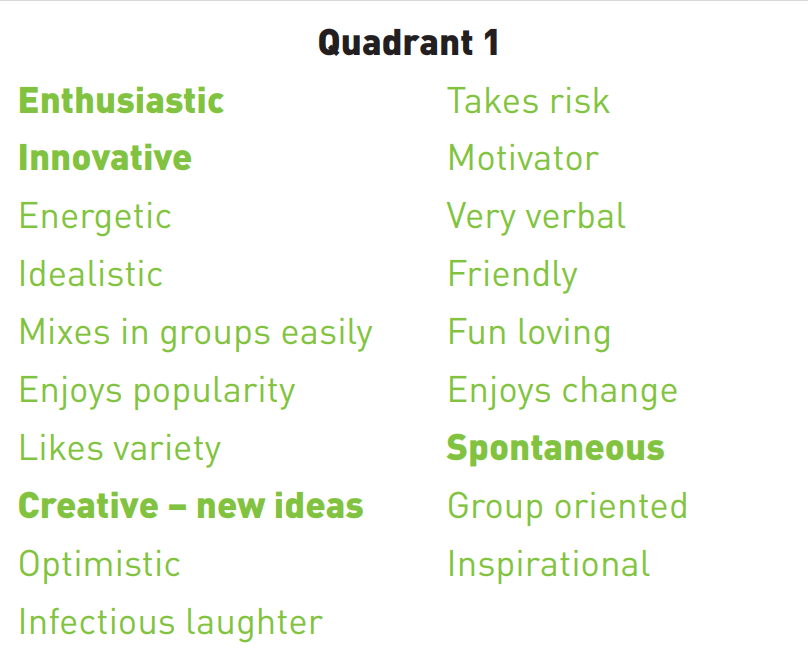
\includegraphics[width=0.8\linewidth]{images/ws1.png}
\end{figure}

\begin{figure}[H]
    \centering
    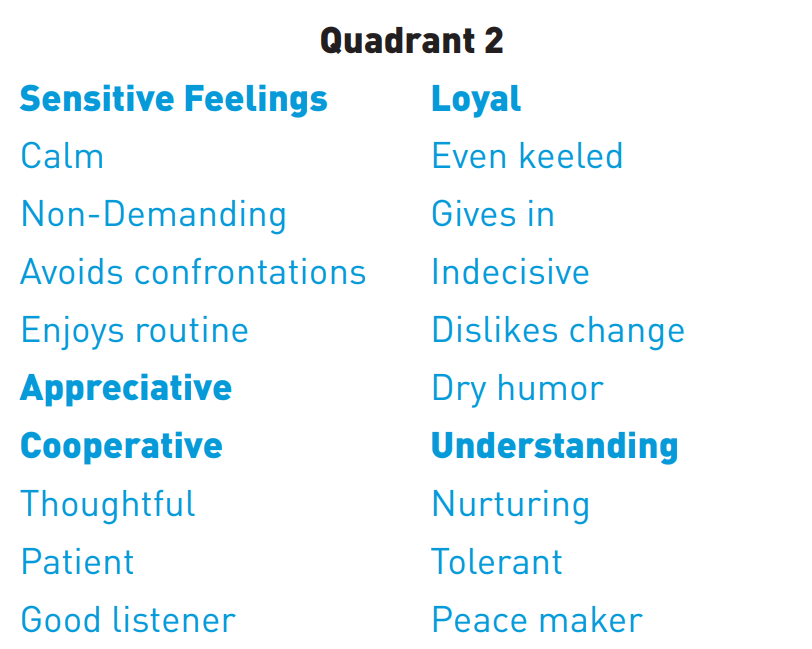
\includegraphics[width=0.8\linewidth]{images/ws2.png}
\end{figure}

\begin{figure}[H]
    \centering
    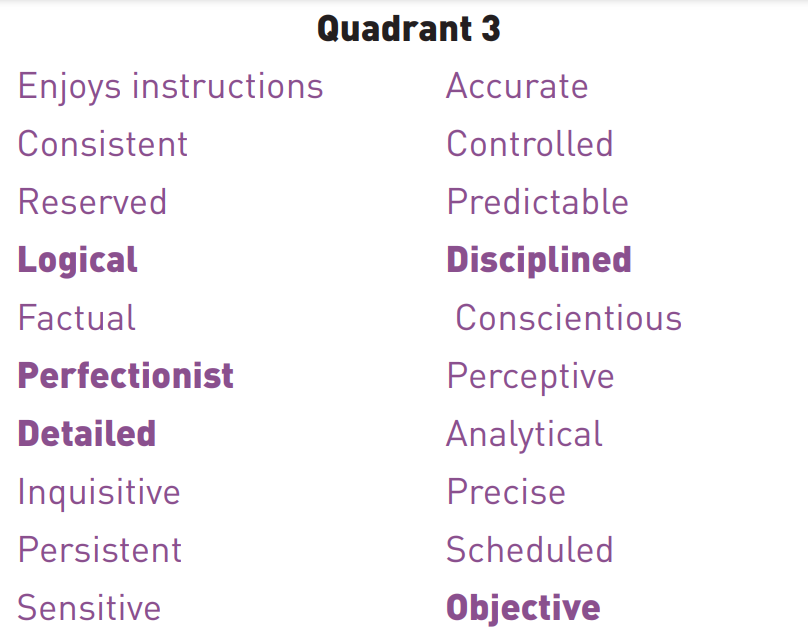
\includegraphics[width=0.8\linewidth]{images/ws3.png}
\end{figure}

\begin{figure}[H]
    \centering
    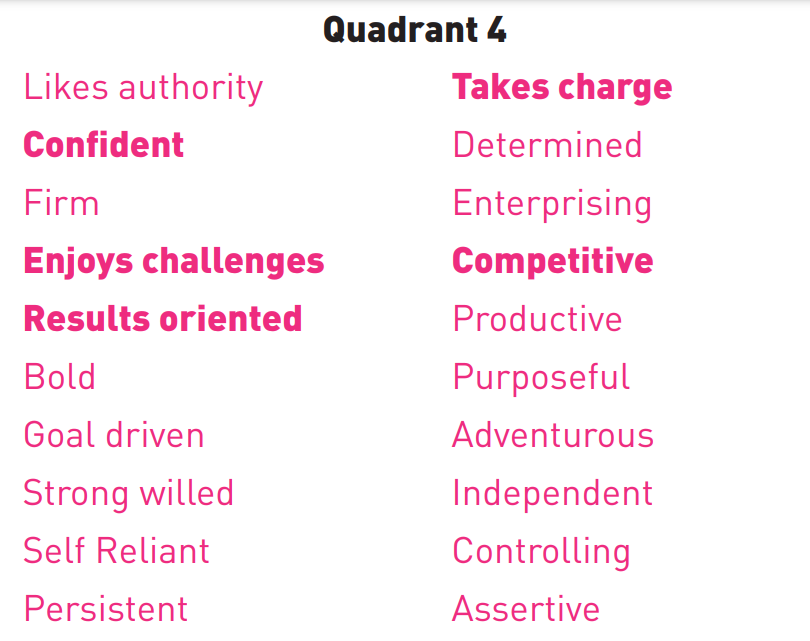
\includegraphics[width=0.8\linewidth]{images/ws4.png}
\end{figure}

\subsection{Trắc nghiệm tính cách True Color}

Bài kiểm tra tính cách True Colors được Don Lowry phát triển vào năm 1978 dựa trên công trình của David Keirsey và Chỉ số loại hình Myers-Briggs (MBTI). Đây là một công cụ đánh giá tính cách nhằm giúp người dùng hiểu rõ hơn về bản thân và người khác bằng cách phân loại tính cách thành bốn màu chính: Xanh Lam, Xanh Lá, Cam và Vàng. Mỗi màu đại diện cho một tập hợp các đặc điểm, giá trị và sở thích riêng biệt.

Bài kiểm tra tính cách True Colors thường được sử dụng để phát triển bản thân và nâng cao khả năng tự nhận thức, giúp người dùng nhận diện điểm mạnh, điểm yếu và sở thích giao tiếp của mình. Việc xác định màu sắc chủ đạo của bản thân sẽ giúp người dùng đưa ra các quyết định sáng suốt hơn trong nhiều lĩnh vực của cuộc sống, chẳng hạn như lựa chọn nghề nghiệp, phát triển mối quan hệ và đặt mục tiêu cá nhân.

Mỗi kết quả màu sắc trong bài kiểm tra True Colors phản ánh những đặc điểm tính cách nổi bật của người dùng. Các màu sắc này có những ý nghĩa đặc biệt sau:

\begin{itemize}
    \item \textbf{Màu Cam:} Đại diện cho sự năng động và phấn khích. Người có màu này thường yêu thích sự vui vẻ, hài hước, dí dỏm và quyến rũ. Họ là những người nhiệt huyết và có khả năng truyền cảm hứng cho người khác.
    \item \textbf{Màu Xanh Lá:} Đại diện cho các hệ thống có trật tự, giống như những gì tìm thấy trong tự nhiên. Người có màu này khát khao tri thức, logic, trí tuệ và có xu hướng tìm kiếm sự hiểu biết sâu sắc về thế giới xung quanh.
    \item \textbf{Màu Xanh Lam:} Đại diện cho cường độ cảm xúc và tâm linh. Người có màu này thích giao tiếp xã hội, luôn tìm cách kết nối với người khác và có khả năng giải quyết xung đột thông qua sự đồng cảm và chia sẻ.
    \item \textbf{Màu Vàng:} Đại diện cho sự chân thực, tin cậy và truyền thống. Người có màu này thích sự trật tự, thống nhất, coi trọng chính trực và trách nhiệm. Họ là những người bạn và đồng nghiệp đáng tin cậy, luôn tôn trọng quy tắc và giá trị cốt lõi.
\end{itemize}

\begin{multicols}{2}
\noindent
\textbf{Câu 1:} Khi đưa ra quyết định: \\
A. Tôi quyết định nhanh chóng theo trực giác đầu tiên. \\
B. Tôi suy nghĩ kỹ, cân nhắc các lựa chọn và sau đó quyết định. \\
C. Tôi lắng nghe cảm xúc của mình và xem xét quyết định của mình sẽ ảnh hưởng đến người khác như thế nào. \\
D. Tôi nghiêm túc và luôn cố gắng đưa ra quyết định đúng đắn. \\

\textbf{Câu 2:} Cách tốt nhất để người khác thể hiện sự quan tâm đến tôi là: \\
A. Làm những điều thú vị với tôi. \\
B. Cho tôi không gian để là chính mình. \\
C. Dành thời gian với tôi, làm bất cứ điều gì. \\
D. Làm những gì tôi muốn; không để tôi thất vọng hoặc không giữ lời. \\

\textbf{Câu 3:} Khi ở bên bạn bè, tôi thích mang đến: \\
A. Sự sôi nổi, niềm vui, những trò đùa. \\
B. Câu hỏi, câu trả lời, một cách nhìn vấn đề logic. \\
C. Sự quan tâm đến người khác, nhiều sự chăm sóc. \\
D. Sự lên kế hoạch, cảm giác an toàn, một chuẩn mực tốt. \\

\textbf{Câu 4:} Tôi thích: \\
A. Hành động ngay lập tức; làm những việc mạo hiểm. \\
B. Cung cấp câu trả lời hoặc suy nghĩ về câu hỏi của mọi người. \\
C. Giúp duy trì sự hài hòa và đoàn kết. \\
D. Có trách nhiệm, đáng tin cậy và giúp đỡ người khác. \\

\textbf{Câu 5:} Một điều mà tôi thực sự giỏi là: \\
A. Hành động dũng cảm. \\
B. Suy nghĩ. \\
C. Nhạy cảm. \\
D. Tổ chức. \\

\textbf{Câu 6:} Bạn bè thân thiết của tôi thường nói rằng tôi là người: \\
A. Cạnh tranh. \\
B. Kín đáo, suy nghĩ sâu sắc. \\
C. Cảm xúc, thân thiện. \\
D. Gọn gàng, chuẩn bị kỹ lưỡng. \\

\textbf{Câu 7:} Quan điểm sống cơ bản của tôi là: \\
A. Sống chậm rãi và tận hưởng từng ngày. \\
B. Tìm hiểu ý nghĩa cuộc sống. \\
C. Giúp đỡ người khác, hạnh phúc và thành công. \\
D. Lên kế hoạch cho tương lai và làm cho nó tốt nhất có thể. \\

\textbf{Câu 8:} Khi tôi cảm thấy chán nản hoặc không vui: \\
A. Tôi thường trở nên thô lỗ, tức giận hoặc thậm chí là xấu tính. \\
B. Tôi thu mình lại, không nói nhiều và cố gắng tự mình suy nghĩ để giải quyết vấn đề. \\
C. Tôi cảm thấy xúc động, buồn và thường thích nói chuyện với người thân. \\
D. Tôi cố gắng tìm ra nguyên nhân của vấn đề và sửa chữa nó. \\

\textbf{Câu 9:} Tôi cảm thấy tốt về bản thân khi: \\
A. Tôi có thể làm những việc khó khăn. \\
B. Tôi có thể giải quyết vấn đề hoặc tìm ra cách giải quyết. \\
C. Tôi có thể giúp đỡ người khác. \\
D. Tôi được đánh giá cao hoặc được khen thưởng vì những việc mình làm. \\

\textbf{Câu 10:} Giáo viên ở trường có thể miêu tả tôi khi tôi hành xử không được tốt và lịch sự là: \\
A. Hỗn láo hoặc hơi hoang dã. \\
B. Kiêu ngạo. \\
C. Nói nhiều. \\
D. Người muốn mọi thứ theo ý mình; thống trị; lo lắng. \\

\textbf{Câu 11:} Giáo viên ở trường (những người thích tôi và tôi học khá tốt trong lớp của họ) có lẽ sẽ mô tả tôi là: \\
A. Dễ thương, một nhà lãnh đạo tự nhiên, thông minh, khiến người khác vui vẻ khi ở cùng. \\
B. Chu đáo, thường có những câu trả lời hay, thích tìm ra vấn đề. \\
C. Tốt bụng, thân thiện, người hòa đồng với các học sinh khác, giúp đỡ giáo viên và những người khác. \\
D. Gọn gàng, ngăn nắp, chuẩn bị kỹ, luôn làm đủ bài tập và là một học sinh giỏi. \\

\end{multicols}

\subsection{Trắc nghiệm thang đo bền chí}

Trắc nghiệm Grit Scale (hay còn gọi là trắc nghiệm về độ bền bỉ) là một công cụ được sử dụng để đo lường sự kiên trì và đam mê của người dùng đối với các mục tiêu dài hạn. Trắc nghiệm này giúp người dùng nhận ra mức độ quyết tâm của mình khi đối mặt với những thử thách khó khăn và khả năng duy trì sự tập trung vào mục tiêu lâu dài.

Bài kiểm tra bao gồm các câu hỏi đánh giá cách người dùng phản ứng với những thất bại, khả năng giữ vững mục tiêu qua thời gian và mức độ người dùng tránh bị phân tâm bởi những mối quan tâm mới. Dựa trên điểm số người dùng đạt được, họ sẽ biết mình có độ kiên trì ở mức độ nào và có thể so sánh với những người khác. Kết quả của bài kiểm tra có thể giúp người dùng hiểu rõ hơn về sức bền của mình trong công việc và học tập.

Căn cứ vào điểm số của người dùng trong từng yếu tố, có thể tham khảo các mức độ sau:

\begin{itemize}
    \item \textbf{Điểm cao trong Grit Scale:} Người dùng là người kiên trì và có khả năng vượt qua các thử thách khó khăn, không dễ dàng bỏ cuộc khi gặp trở ngại.
    \item \textbf{Điểm trung bình trong Grit Scale:} Người dùng có khả năng kiên trì ở mức vừa phải, nhưng đôi khi có thể bị phân tâm bởi những sở thích hoặc mục tiêu mới.
    \item \textbf{Điểm thấp trong Grit Scale:} Người dùng có thể dễ bị mất hứng thú và khó giữ vững mục tiêu lâu dài khi gặp phải khó khăn.
\end{itemize}

\begin{multicols}{2}
\noindent
\textbf{Câu 1:} Tôi đã vượt qua những trở ngại để chinh phục một thử thách quan trọng. \\
A. Rất giống tôi \\
B. Khá giống tôi \\
C. Hơi giống tôi \\
D. Không giống tôi lắm \\
E. Hoàn toàn không giống tôi \\

\textbf{Câu 2:} Ý tưởng và dự án mới đôi khi làm tôi mất tập trung vào những cái trước đó. \\
A. Rất giống tôi \\
B. Khá giống tôi \\
C. Hơi giống tôi \\
D. Không giống tôi lắm \\
E. Hoàn toàn không giống tôi \\

\textbf{Câu 3:} Sở thích của tôi thay đổi theo từng năm. \\
A. Rất giống tôi \\
B. Khá giống tôi \\
C. Hơi giống tôi \\
D. Không giống tôi lắm \\
E. Hoàn toàn không giống tôi \\

\textbf{Câu 4:} Những trở ngại không làm tôi nản lòng. \\
A. Rất giống tôi \\
B. Khá giống tôi \\
C. Hơi giống tôi \\
D. Không giống tôi lắm \\
E. Hoàn toàn không giống tôi \\

\textbf{Câu 5:} Tôi đã từng bị cuốn hút bởi một ý tưởng hoặc dự án trong thời gian ngắn nhưng sau đó mất hứng thú. \\
A. Rất giống tôi \\
B. Khá giống tôi \\
C. Hơi giống tôi \\
D. Không giống tôi lắm \\
E. Hoàn toàn không giống tôi \\

\textbf{Câu 6:} Tôi là một người làm việc chăm chỉ. \\
A. Rất giống tôi \\
B. Khá giống tôi \\
C. Hơi giống tôi \\
D. Không giống tôi lắm \\
E. Hoàn toàn không giống tôi \\

\textbf{Câu 7:} Tôi thường đặt ra một mục tiêu nhưng sau đó lại chọn theo đuổi một mục tiêu khác. \\
A. Rất giống tôi \\
B. Khá giống tôi \\
C. Hơi giống tôi \\
D. Không giống tôi lắm \\
E. Hoàn toàn không giống tôi \\

\textbf{Câu 8:} Tôi gặp khó khăn trong việc duy trì tập trung vào các dự án kéo dài hơn vài tháng. \\
A. Rất giống tôi \\
B. Khá giống tôi \\
C. Hơi giống tôi \\
D. Không giống tôi lắm \\
E. Hoàn toàn không giống tôi \\

\textbf{Câu 9:} Tôi hoàn thành mọi thứ tôi bắt đầu. \\
A. Rất giống tôi \\
B. Khá giống tôi \\
C. Hơi giống tôi \\
D. Không giống tôi lắm \\
E. Hoàn toàn không giống tôi \\

\textbf{Câu 10:} Tôi đã đạt được một mục tiêu mà phải mất nhiều năm để hoàn thành. \\
A. Rất giống tôi \\
B. Khá giống tôi \\
C. Hơi giống tôi \\
D. Không giống tôi lắm \\
E. Hoàn toàn không giống tôi \\

\textbf{Câu 11:} Tôi hứng thú với những điều mới mẻ mỗi vài tháng. \\
A. Rất giống tôi \\
B. Khá giống tôi \\
C. Hơi giống tôi \\
D. Không giống tôi lắm \\
E. Hoàn toàn không giống tôi \\

\textbf{Câu 12:} Tôi là một người kiên trì. \\
A. Rất giống tôi \\
B. Khá giống tôi \\
C. Hơi giống tôi \\
D. Không giống tôi lắm \\
E. Hoàn toàn không giống tôi \\

\end{multicols}


